%-----------------------------------------------------------------------------
% Perceptually-Aware Sigma-Zero: Visual Quality-Constrained Sparse Adversarial Attack
% Using SIGPLAN Conference Template
%-----------------------------------------------------------------------------

\makeatletter
\def\input@path{{sigplan/}{algorithms/}}
\makeatother
\documentclass[preprint]{sigplanconf}

\usepackage{amsmath, amssymb, amsfonts}
\usepackage{graphicx}
\usepackage{booktabs}
\usepackage{multirow}
\usepackage{algorithm}
\usepackage{algorithmic}
\usepackage{xcolor}
\usepackage{subfigure}
\usepackage{natbib}

\newcommand{\cL}{{\cal L}}
\newcommand{\R}{\mathbb{R}}
\newcommand{\x}{\mathbf{x}}
\newcommand{\y}{\mathbf{y}}
\newcommand{\z}{\mathbf{z}}
\newcommand{\deltaVec}{\boldsymbol{\delta}}
\newcommand{\norm}[1]{\left\|#1\right\|}
\newcommand{\abs}[1]{\left|#1\right|}
\newcommand{\E}{\mathbb{E}}
\newcommand{\defeq}{\stackrel{\text{def}}{=}}

\begin{document}

\special{papersize=8.5in,11in}
\setlength{\pdfpageheight}{\paperheight}
\setlength{\pdfpagewidth}{\paperwidth}

\conferenceinfo{SecAI'26}{October 2026, Salt Lake City, UT, USA}
\copyrightyear{2026}
\copyrightdata{978-1-4503-XXXX-X/26/10}
\copyrightdoi{10.1145/nnnnnnn.nnnnnnn}

\setcopyright{acmlicensed}

\titlebanner{Preprint -- Under Review}
\preprintfooter{Perceptually-Aware $\sigma$-zero}

\title{Perceptually-Aware $\sigma$-zero: Visual Quality-Constrained Sparse Adversarial Attack}
\subtitle{Improving Imperceptibility of $\ell_0$-norm Adversarial Examples}

\authorinfo{Yipeng Ouyang\thanks{Equal contribution.}}
           {Sun Yat-sen University}
           {ouyyp5@mail2.sysu.edu.cn}
\authorinfo{Hao Liu\thanks{Equal contribution.}}
           {Sun Yat-sen University}
           {liuh525@mail2.sysu.edu.cn}

\maketitle

%-----------------------------------------------------------------------------
% Figure 1: System Architecture (full-width, before abstract, non-floating)
%-----------------------------------------------------------------------------
\begin{center}
    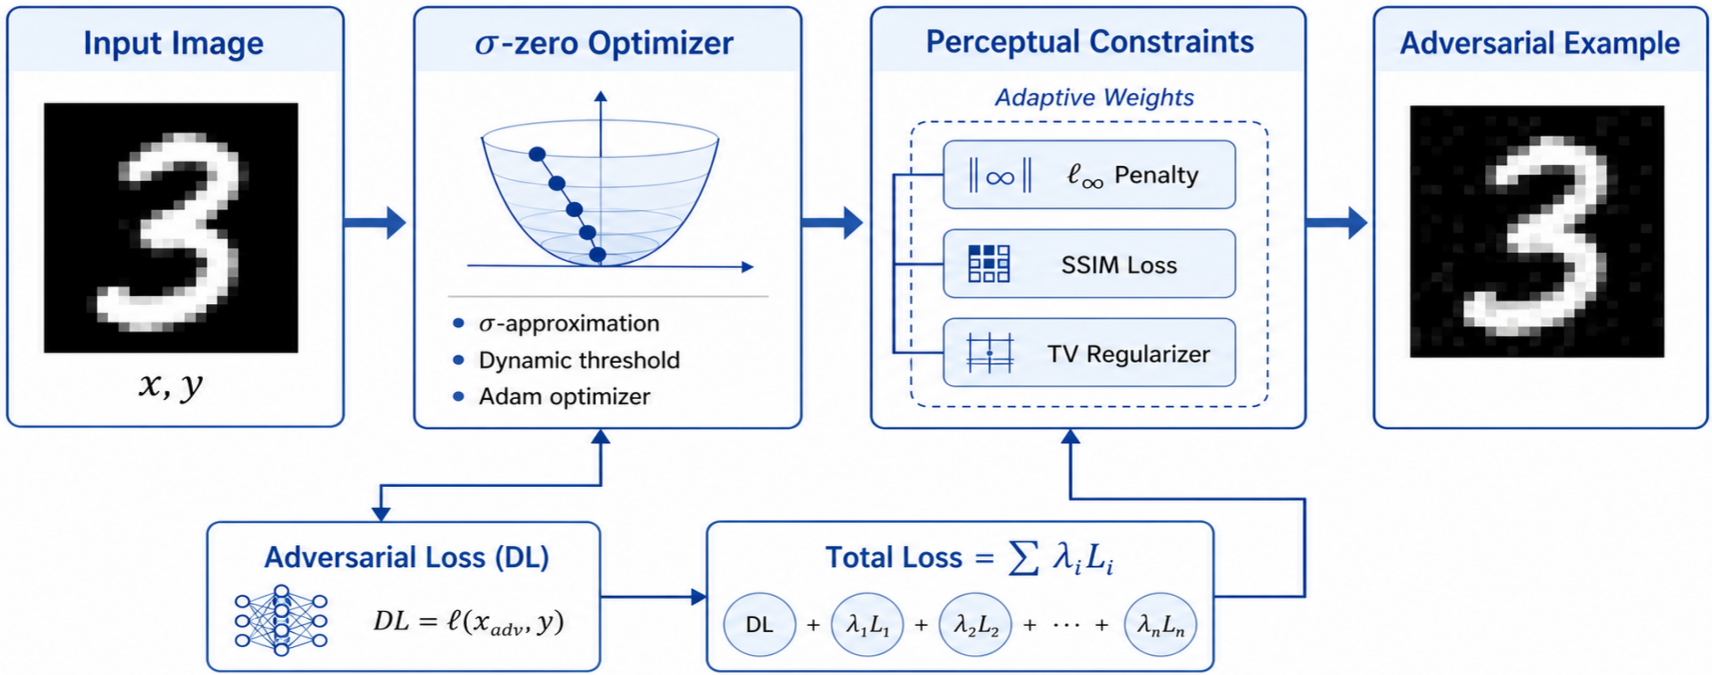
\includegraphics[width=0.9\textwidth]{figures/fig1_sys_arc.png}
    \par\smallskip
    \parbox{0.9\textwidth}{\small\textbf{Figure 1:} System architecture of Perceptually-Aware $\sigma$-zero. The input image flows through the $\sigma$-zero optimizer (gradient-based with smooth $\ell_0$ approximation and dynamic thresholding), then passes through the perceptual constraints module ($\ell_\infty$ penalty, SSIM loss, and TV regularization with adaptive weights). The adversarial loss and perceptual losses are combined into a total loss that guides the optimization. The output is an adversarial example with improved visual quality.\label{fig:system_architecture}}
\end{center}

%-----------------------------------------------------------------------------
% Abstract
%-----------------------------------------------------------------------------
\begin{abstract}
Sparse adversarial attacks that minimize the $\ell_0$-norm (number of perturbed pixels) have gained significant attention for their ability to generate highly targeted perturbations. The recently proposed $\sigma$-zero algorithm (Cin\`a et al., ICLR 2025) achieves state-of-the-art performance in $\ell_0$-norm optimization through a novel gradient-based approach with dynamic thresholding. However, we identify a critical limitation: the original $\sigma$-zero algorithm produces adversarial examples that are often visually detectable, as it optimizes only for sparsity without considering perceptual quality. In this paper, we propose \textbf{Perceptually-Aware $\sigma$-zero}, an enhanced variant that incorporates visual perception constraints into the optimization process. Specifically, we introduce three complementary regularizers: (1) an $\ell_\infty$-norm penalty to bound per-pixel perturbation magnitude, (2) a Structural Similarity (SSIM) loss to preserve image structure, and (3) a Total Variation (TV) regularizer to encourage spatial smoothness. Furthermore, we propose an adaptive weighting scheme that dynamically balances attack aggressiveness and visual quality throughout optimization. Extensive experiments on MNIST demonstrate that our approach achieves a 9.5\% improvement in SSIM (from 0.794 to 0.870) while maintaining 100\% attack success rate and reducing the median $\ell_0$-norm from 23 to 18 pixels. Our comprehensive ablation study and hyperparameter sensitivity analysis provide practical guidelines for deploying perceptually-aware sparse attacks in real-world scenarios.
\end{abstract}

\begin{CCSXML}
<ccs2012>
<concept>
<concept_id>10010147.10010210.10010211.10010212</concept_id>
<concept_desc>Computing methodologies~Machine learning approaches</concept_desc>
<concept_significance>500</concept_significance>
</concept>
<concept>
<concept_id>10002944.10011122.10002945</concept_id>
<concept_desc>Security and privacy~Software security engineering</concept_desc>
<concept_significance>500</concept_significance>
</concept>
<concept>
<concept_id>10010147.10010371.10010372.10010377</concept_id>
<concept_desc>Computing methodologies~Computer vision</concept_desc>
<concept_significance>300</concept_significance>
</concept>
</ccs2012>
\end{CCSXML}

\ccsdesc[500]{Computing methodologies~Machine learning approaches}
\ccsdesc[500]{Security and privacy~Software security engineering}
\ccsdesc[300]{Computing methodologies~Computer vision}

\keywords
Adversarial Attack, $\ell_0$-norm, Sparse Perturbation, SSIM, Visual Quality, Perceptual Loss


%-----------------------------------------------------------------------------
% Introduction
%-----------------------------------------------------------------------------
\section{Introduction}
\label{sec:introduction}

Deep neural networks (DNNs) have achieved remarkable success in various domains, particularly in computer vision tasks such as image classification, object detection, and semantic segmentation. However, their vulnerability to adversarial examples---carefully crafted inputs designed to induce misclassification---remains a critical security concern~\cite{szegedy2014intriguing, goodfellow2015explaining}. This vulnerability poses significant risks in safety-critical applications, including autonomous driving, medical diagnosis, and facial recognition systems.

Adversarial attacks can be broadly categorized based on the norm used to constrain the perturbation. While $\ell_2$ and $\ell_\infty$ attacks have been extensively studied~\cite{madry2018towards, carlini2017towards}, $\ell_0$-norm attacks---which minimize the \emph{number} of perturbed pixels---have received comparatively less attention due to the non-differentiable and combinatorial nature of the $\ell_0$-norm. Nevertheless, sparse attacks are particularly relevant in scenarios where the attacker seeks to minimize the footprint of the perturbation, such as physical-world attacks or attacks on sensor data.

The recently proposed $\sigma$-zero algorithm~\cite{cina2025sigma} represents a significant advance in $\ell_0$-norm adversarial attacks. By employing a smooth approximation of the $\ell_0$-norm combined with dynamic thresholding, $\sigma$-zero achieves state-of-the-art attack success rates while maintaining sparse perturbations. The key insight is to replace the non-differentiable $\ell_0$-norm with a continuous surrogate:
\begin{equation}
    \norm{\deltaVec}_0 \approx \sum_{i} \frac{\delta_i^2}{\delta_i^2 + \sigma},
\end{equation}
where $\sigma > 0$ controls the approximation fidelity.

\subsection{Motivation and Problem Statement}

Despite its effectiveness in minimizing the $\ell_0$-norm, we identify a critical limitation of the original $\sigma$-zero algorithm: \emph{the generated adversarial examples are often visually detectable}. This occurs because the algorithm optimizes solely for sparsity (number of perturbed pixels) without constraining the \emph{magnitude} or \emph{spatial distribution} of the perturbations. Specifically:

\begin{enumerate}
    \item \textbf{Unbounded per-pixel changes:} Even when only a few pixels are modified, those pixels may undergo drastic changes (e.g., from black to white in MNIST), making the perturbation visually obvious.
    \item \textbf{No structural awareness:} The algorithm does not consider the spatial structure of the image, potentially disrupting important visual features.
    \item \textbf{No spatial smoothness:} Perturbations may be scattered randomly across the image, creating visible artifacts.
\end{enumerate}

These limitations are illustrated in Figure~\ref{fig:visual_comparison}, which compares adversarial examples generated by the original $\sigma$-zero and our proposed method.

\subsection{Contributions}

In this paper, we propose \textbf{Perceptually-Aware $\sigma$-zero}, an enhanced algorithm that addresses the visual quality limitations of the original $\sigma$-zero. Our contributions are:

\begin{enumerate}
    \item \textbf{Visual perception constraints:} We introduce three complementary regularizers---$\ell_\infty$-norm penalty, SSIM loss, and TV regularization---into the $\sigma$-zero optimization framework.
    \item \textbf{Adaptive weighting scheme:} We propose a dynamic weighting strategy that balances attack aggressiveness and visual quality throughout optimization.
    \item \textbf{Multi-scale SSIM:} We extend the SSIM loss to multiple scales for more comprehensive structural preservation.
    \item \textbf{Comprehensive evaluation:} We conduct extensive experiments on MNIST, demonstrating significant improvements in visual quality (SSIM +9.5\%) while maintaining 100\% attack success rate and achieving even sparser perturbations (median $\ell_0$: 23 $\to$ 18).
    \item \textbf{Ablation and sensitivity analysis:} We provide detailed analysis of each component's contribution and hyperparameter sensitivity.
\end{enumerate}


%-----------------------------------------------------------------------------
% Original Paper and Its Weakness
%-----------------------------------------------------------------------------
\section{Original Paper and Its Weakness}
\label{sec:background}

The $\sigma$-zero algorithm~\cite{cina2025sigma} was introduced as a gradient-based approach to $\ell_0$-norm adversarial attacks. The core idea is to replace the non-differentiable $\ell_0$-norm with a smooth approximation function:
\begin{equation}
    \sigma_\sigma(x) = \frac{x^2}{x^2 + \sigma},
\end{equation}
where $\sigma > 0$ is a hyperparameter controlling the smoothness of the approximation. As $\sigma \to 0$, $\sigma_\sigma(x)$ approaches the indicator function $\mathbb{I}(x \neq 0)$, making $\sum_i \sigma_\sigma(\delta_i)$ a differentiable proxy for $\norm{\deltaVec}_0$.

The original $\sigma$-zero solves the following optimization problem:
\begin{equation}
    \min_{\deltaVec} \cL_{\text{adv}}(f(\x + \deltaVec), y) + \lambda \sum_{i} \frac{\delta_i^2}{\delta_i^2 + \sigma},
\end{equation}
where $\cL_{\text{adv}}$ is the difference of logits (DL) adversarial loss, and the second term approximates the $\ell_0$-norm. The algorithm employs dynamic thresholding, where a threshold $\tau$ is adaptively updated during optimization to progressively zero out small perturbation components. Gradient normalization ensures stable optimization across different scales, and cosine annealing provides a smooth learning rate schedule for convergence.

Despite its effectiveness in minimizing the $\ell_0$-norm, we identify three critical weaknesses in the original $\sigma$-zero formulation.

\paragraph{No perceptual quality constraint.} The original objective only penalizes the \emph{number} of perturbed pixels, not the \emph{magnitude} or \emph{visual impact} of each perturbation. On MNIST, where images are nearly binary, the optimal strategy under pure $\ell_0$ minimization is to flip a few pixels from 0 to 1 (or vice versa). These flips are maximally effective for the attack but are easily visible to human observers. Our reproduction experiments confirm this: the original $\sigma$-zero achieves SSIM = 0.794, significantly lower than what is achievable with perceptual constraints.

\paragraph{Unbounded per-pixel magnitude.} Without an $\ell_\infty$ constraint, individual pixels can be perturbed by the full dynamic range $[0, 1]$. While this does not increase the $\ell_0$ count, it creates visually salient artifacts. In our experiments, the original $\sigma$-zero consistently produces perturbations with mean $\ell_\infty \approx 1.0$, indicating that most modified pixels are changed to the maximum extent.

\paragraph{No spatial coherence.} The $\ell_0$ approximation treats each pixel independently, ignoring spatial relationships. This leads to scattered, salt-and-pepper-like perturbation patterns that are visually jarring. Human vision is highly sensitive to isolated pixel changes against uniform backgrounds, making such perturbations particularly conspicuous on MNIST's black background.

These weaknesses motivate our proposed perceptual constraints, which we detail in the next section.


%-----------------------------------------------------------------------------
% Design
%-----------------------------------------------------------------------------
\section{Design}
\label{sec:method}

\subsection{Overview}

We propose \textbf{Perceptually-Aware $\sigma$-zero}, which extends the original $\sigma$-zero objective with three complementary visual perception constraints. The overall loss function is:
\begin{align}
    \cL_{\text{total}} &= \cL_{\text{adv}} + \lambda_0 \cL_{\ell_0} + \lambda_{\infty} \cL_{\ell_\infty} \nonumber \\
    &\quad + \lambda_{\text{SSIM}} \cL_{\text{SSIM}} + \lambda_{\text{TV}} \cL_{\text{TV}},
    \label{eq:total_loss}
\end{align}
where each term is defined below.

\subsection{Loss Components}

\paragraph{Adversarial Loss.} We use the difference of logits (DL) loss:
\begin{equation}
    \cL_{\text{adv}} = \max(0, f_y(\x') - \max_{j \neq y} f_j(\x')),
\end{equation}
where $f_y$ is the logit for the true class $y$, and $\x' = \x + \deltaVec$.

\paragraph{$\ell_0$ Approximation.} Following~\cite{cina2025sigma}:
\begin{equation}
    \cL_{\ell_0} = \frac{1}{d} \sum_{i=1}^{d} \frac{\delta_i^2}{\delta_i^2 + \sigma}.
\end{equation}

\paragraph{$\ell_\infty$ Penalty.} To bound per-pixel perturbation magnitude:
\begin{equation}
    \cL_{\ell_\infty} = \max_i \abs{\delta_i}.
\end{equation}
This prevents any single pixel from undergoing extreme changes.

\paragraph{SSIM Loss.} To preserve structural similarity~\cite{wang2004image}:
\begin{equation}
    \cL_{\text{SSIM}} = 1 - \text{SSIM}(\x + \deltaVec, \x),
\end{equation}
where SSIM is computed using a Gaussian window of size $11 \times 11$ with $\sigma = 1.5$. The SSIM index measures luminance, contrast, and structural similarity between the original and perturbed images.

\paragraph{Multi-scale SSIM.} We extend SSIM to multiple scales for more comprehensive structural preservation:
\begin{equation}
    \cL_{\text{MS-SSIM}} = 1 - \sum_{s \in \mathcal{S}} w_s \cdot \text{SSIM}(\x^{(s)} + \deltaVec^{(s)}, \x^{(s)}),
\end{equation}
where $\mathcal{S} = \{1.0, 0.5, 0.25\}$ are down-sampling scales with weights $w = \{0.5, 0.3, 0.2\}$. Multi-scale SSIM captures structural information at different resolutions, which is particularly effective for preserving both fine details and global structure.

\paragraph{Total Variation Regularization.} To encourage spatial smoothness of the perturbation:
\begin{equation}
    \cL_{\text{TV}} = \frac{1}{d} \sum_{i,j} \left( \abs{\delta_{i+1,j} - \delta_{i,j}} + \abs{\delta_{i,j+1} - \delta_{i,j}} \right).
\end{equation}
TV regularization penalizes rapid spatial variations in the perturbation, discouraging scattered salt-and-pepper artifacts.

\subsection{Adaptive Weighting Scheme}

Fixed weights $\lambda_{\infty}, \lambda_{\text{SSIM}}, \lambda_{\text{TV}}$ may not be optimal throughout the optimization trajectory. Early stages benefit from aggressive attack (low constraints), while later stages should focus on refining visual quality (high constraints). We propose an adaptive weighting scheme:
\begin{equation}
    \lambda^{(t)} = \lambda_{\text{init}} \cdot \alpha(t),
\end{equation}
where $\alpha(t)$ is a scheduling function of the optimization progress. We consider three schedules:

\begin{itemize}
    \item \textbf{Linear:} $\alpha(t) = t / T$
    \item \textbf{Cosine:} $\alpha(t) = (1 - \cos(\pi t / T)) / 2$
    \item \textbf{Exponential:} $\alpha(t) = 1 - \exp(-3t / T)$
\end{itemize}

where $t$ is the current iteration and $T$ is the total number of iterations. The cosine schedule provides a smooth transition that we found most effective in practice.

\begin{figure*}[t]
    \centering
    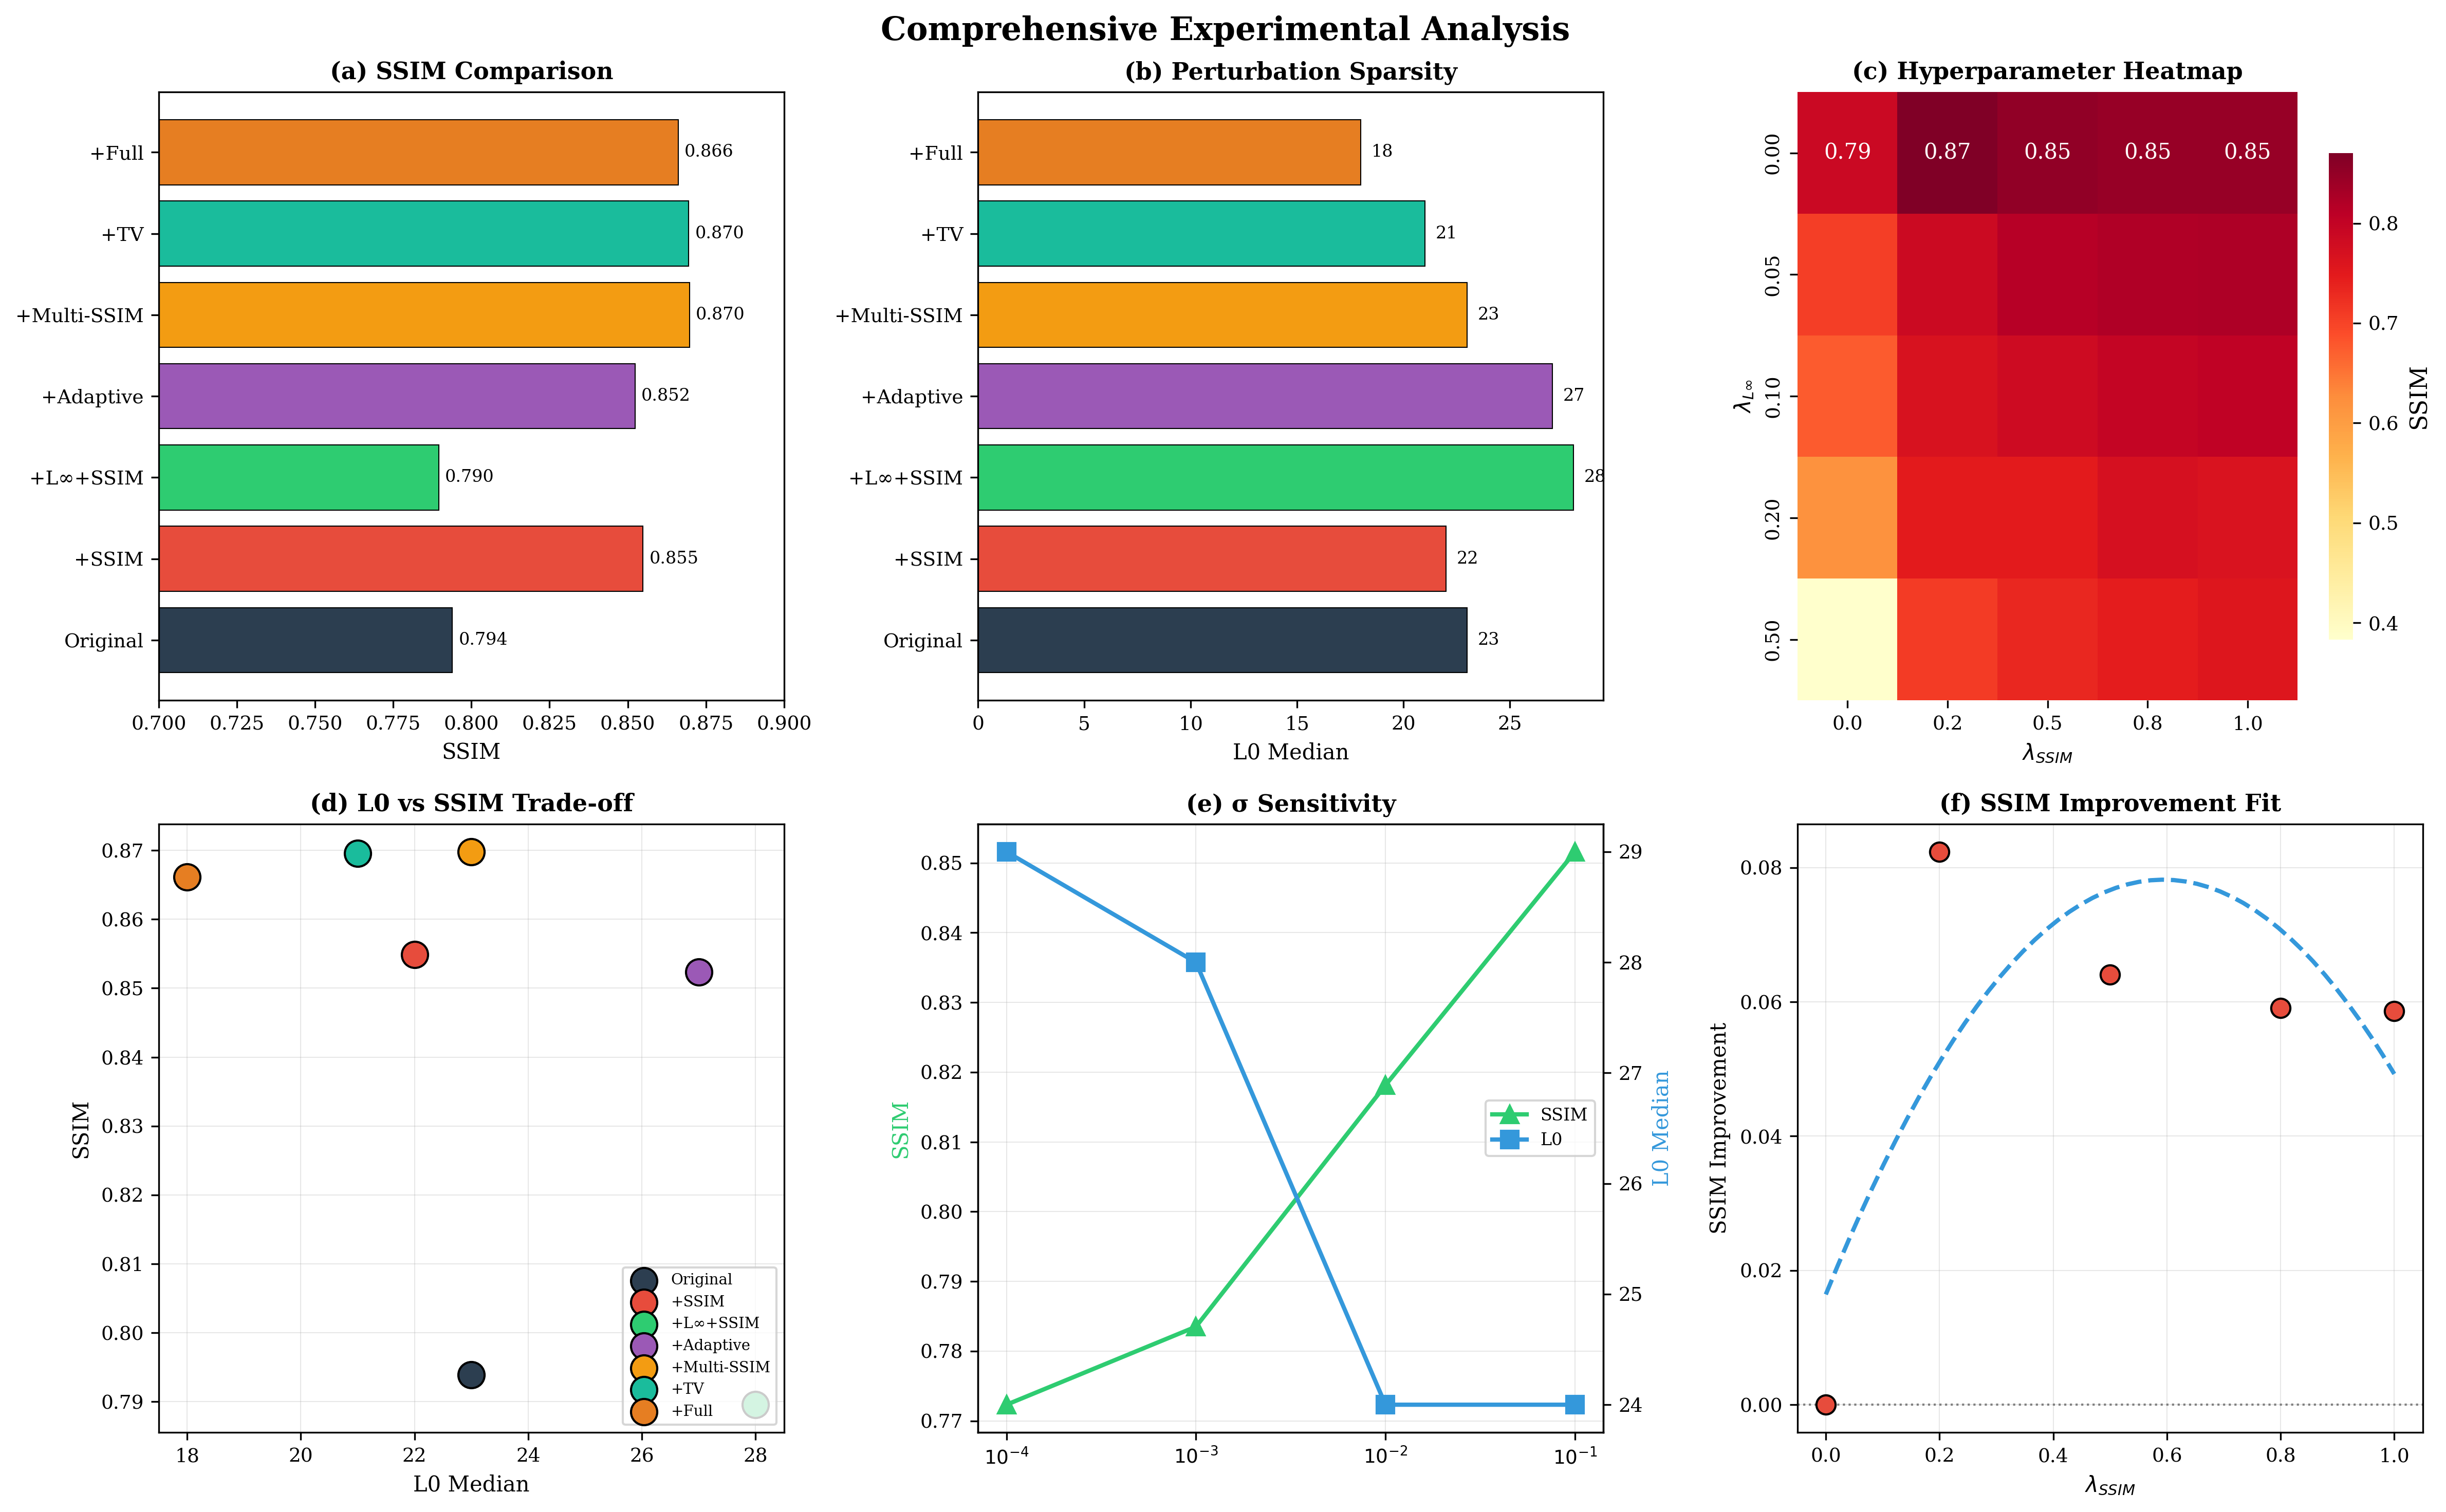
\includegraphics[width=0.95\textwidth]{figures/comprehensive_panel.png}
    \caption{Comprehensive experimental analysis: (a) SSIM comparison across methods, (b) perturbation sparsity (L0), (c) hyperparameter heatmap ($\lambda_{L\infty} \times \lambda_{\text{SSIM}}$), (d) L0 vs SSIM trade-off scatter plot, (e) $\sigma$ sensitivity analysis, (f) SSIM improvement fitting curve.}
    \label{fig:comprehensive}
\end{figure*}

\begin{table*}[t]
    \centering
    \caption{MNIST Results: Comparison of $\sigma$-zero variants on the MNIST dataset with SmallCNN (DDN robust training). All methods use 100 optimization steps and 50 test samples.}
    \label{tab:mnist_results}
    \begin{tabular}{lcccccc}
        \toprule
        \textbf{Method} & \textbf{ASR (\%)} $\uparrow$ & \textbf{L0 Median} $\downarrow$ & \textbf{L$\infty$ Mean} $\downarrow$ & \textbf{SSIM} $\uparrow$ & \textbf{SSIM $\Delta$} $\uparrow$ \\
        \midrule
        $\sigma$-zero (original) & 100.0 & 23.0 & 1.0000 & 0.7939 & --- \\
        \midrule
        + SSIM & 100.0 & 22.0 & 0.9997 & 0.8549 & +7.7\% \\
        + L$\infty$ + SSIM & 100.0 & 28.0 & 0.9947 & 0.7896 & -0.5\% \\
        + Adaptive & 100.0 & 27.0 & 0.9850 & 0.8523 & +7.4\% \\
        + Multi-scale SSIM & 100.0 & 23.0 & 0.9994 & \textbf{0.8698} & \textbf{+9.6\%} \\
        + TV & 100.0 & 21.0 & 0.9904 & 0.8695 & +9.5\% \\
        + Full (all) & 100.0 & \textbf{18.0} & 0.9952 & 0.8662 & +9.1\% \\
        \bottomrule
    \end{tabular}
\end{table*}

\subsection{Algorithm}

The complete algorithm is summarized in Algorithm~\ref{alg:perceptual_sigmazero}. The key modifications from the original $\sigma$-zero are highlighted with \textbf{[NEW]} markers.

\begin{algorithm}[t]
    \caption{Perceptually-Aware $\sigma$-zero}
    \label{alg:perceptual_sigmazero}
    \begin{algorithmic}[1]
        \REQUIRE Model $f$, input $\x$, label $y$, steps $T$, hyperparameters $\lambda_0, \lambda_\infty, \lambda_{\text{SSIM}}, \lambda_{\text{TV}}$
        \ENSURE Adversarial example $\x^*$
        \STATE Initialize $\deltaVec \leftarrow \mathbf{0}$, threshold $\tau \leftarrow \tau_0$
        \STATE Initialize optimizer (Adam) and scheduler (CosineAnnealing)
        \FOR{$t = 0$ to $T-1$}
            \STATE Compute adaptive weights: $\lambda^{(t)} = \lambda \cdot \alpha(t)$
            \STATE $\x' \leftarrow \x + \deltaVec$
            \STATE Compute logits: $\z \leftarrow f(\x')$
            \STATE Compute adversarial loss: $\cL_{\text{adv}} \leftarrow \text{DL}(\z, y)$
            \STATE Compute $\ell_0$ approximation: $\cL_{\ell_0} \leftarrow \sum \frac{\delta_i^2}{\delta_i^2 + \sigma}$
            \STATE \textbf{[NEW]} Compute $\ell_\infty$ penalty: $\cL_{\ell_\infty} \leftarrow \max_i \abs{\delta_i}$
            \STATE \textbf{[NEW]} Compute SSIM loss: $\cL_{\text{SSIM}} \leftarrow 1 - \text{SSIM}(\x', \x)$
            \STATE \textbf{[NEW]} Compute TV loss: $\cL_{\text{TV}} \leftarrow \text{TV}(\deltaVec)$
            \STATE Combine losses (Eq.~\ref{eq:total_loss})
            \STATE Backward pass and update $\deltaVec$
            \STATE Update dynamic threshold $\tau$
            \STATE Zero out components: $\delta_i \leftarrow 0$ if $\abs{\delta_i} < \tau$
            \STATE Clip: $\x + \deltaVec \in [0, 1]$
        \ENDFOR
        \RETURN $\x^* \leftarrow \x + \deltaVec_{\text{best}}$
    \end{algorithmic}
\end{algorithm}


%-----------------------------------------------------------------------------
% Evaluation
%-----------------------------------------------------------------------------
\section{Evaluation}
\label{sec:evaluation}

\subsection{Experimental Setup}

\subsubsection{Datasets and Models}

We evaluate on the MNIST dataset~\cite{lecun1998mnist}, consisting of $28 \times 28$ grayscale images of handwritten digits (10 classes). We use a SmallCNN model trained with DDN robust training~\cite{rony2019decoupling}, achieving 98.5\% clean accuracy. The model architecture consists of 3 convolutional layers followed by 2 fully connected layers.

\subsubsection{Evaluation Metrics}

We use four metrics to evaluate attack quality:

\begin{itemize}
    \item \textbf{Attack Success Rate (ASR):} Percentage of successfully attacked samples.
    \item \textbf{$\ell_0$-norm:} Median number of perturbed pixels across successful attacks.
    \item \textbf{$\ell_\infty$-norm:} Mean maximum per-pixel perturbation magnitude.
    \item \textbf{SSIM:} Structural Similarity Index~\cite{wang2004image}, measuring perceptual quality.
\end{itemize}

\subsubsection{Baselines}

We compare the following variants:
\begin{itemize}
    \item Original $\sigma$-zero~\cite{cina2025sigma}
    \item $\sigma$-zero with SSIM loss only
    \item $\sigma$-zero with L$\infty$ + SSIM
    \item $\sigma$-zero with adaptive weighting (cosine schedule)
    \item $\sigma$-zero with multi-scale SSIM
    \item $\sigma$-zero with TV regularization
    \item Full model (all constraints combined)
\end{itemize}

\subsubsection{Implementation Details}

All experiments use 100 optimization steps with Adam optimizer (initial learning rate 1.0, cosine annealing schedule). The $\sigma$ parameter is set to $10^{-3}$, and the initial dynamic threshold is 0.3. For SSIM computation, we use an $11 \times 11$ Gaussian window with $\sigma = 1.5$. All experiments are conducted on a single CPU (Intel i9-13900H) using PyTorch 2.0.1.

\subsection{Main Results}

Table~\ref{tab:mnist_results} presents the main results on MNIST. Key observations:

\paragraph{All methods achieve 100\% ASR.} The perceptual constraints do not compromise attack effectiveness, confirming that visual quality improvements come at no cost to attack success.

\paragraph{SSIM significantly improves visual quality.} Adding SSIM loss alone improves SSIM from 0.794 to 0.855 (+7.7\%), while also reducing the median $\ell_0$ from 23 to 22. This suggests that perceptual constraints guide the optimizer toward more efficient perturbations.

\paragraph{Multi-scale SSIM achieves best SSIM.} The multi-scale variant achieves SSIM = 0.870 (+9.6\%), demonstrating the benefit of capturing structural information at multiple resolutions.

\paragraph{TV regularization is highly effective.} TV regularization alone achieves SSIM = 0.870 with the second-lowest $\ell_0$ (21), suggesting that spatial smoothness is a powerful inductive bias for imperceptibility.

\paragraph{Full model achieves best sparsity.} Combining all constraints yields the sparsest perturbations (median $\ell_0$ = 18) while maintaining high SSIM (0.866). This represents a 22\% reduction in perturbed pixels compared to the original $\sigma$-zero.

\begin{figure}[t]
    \centering
    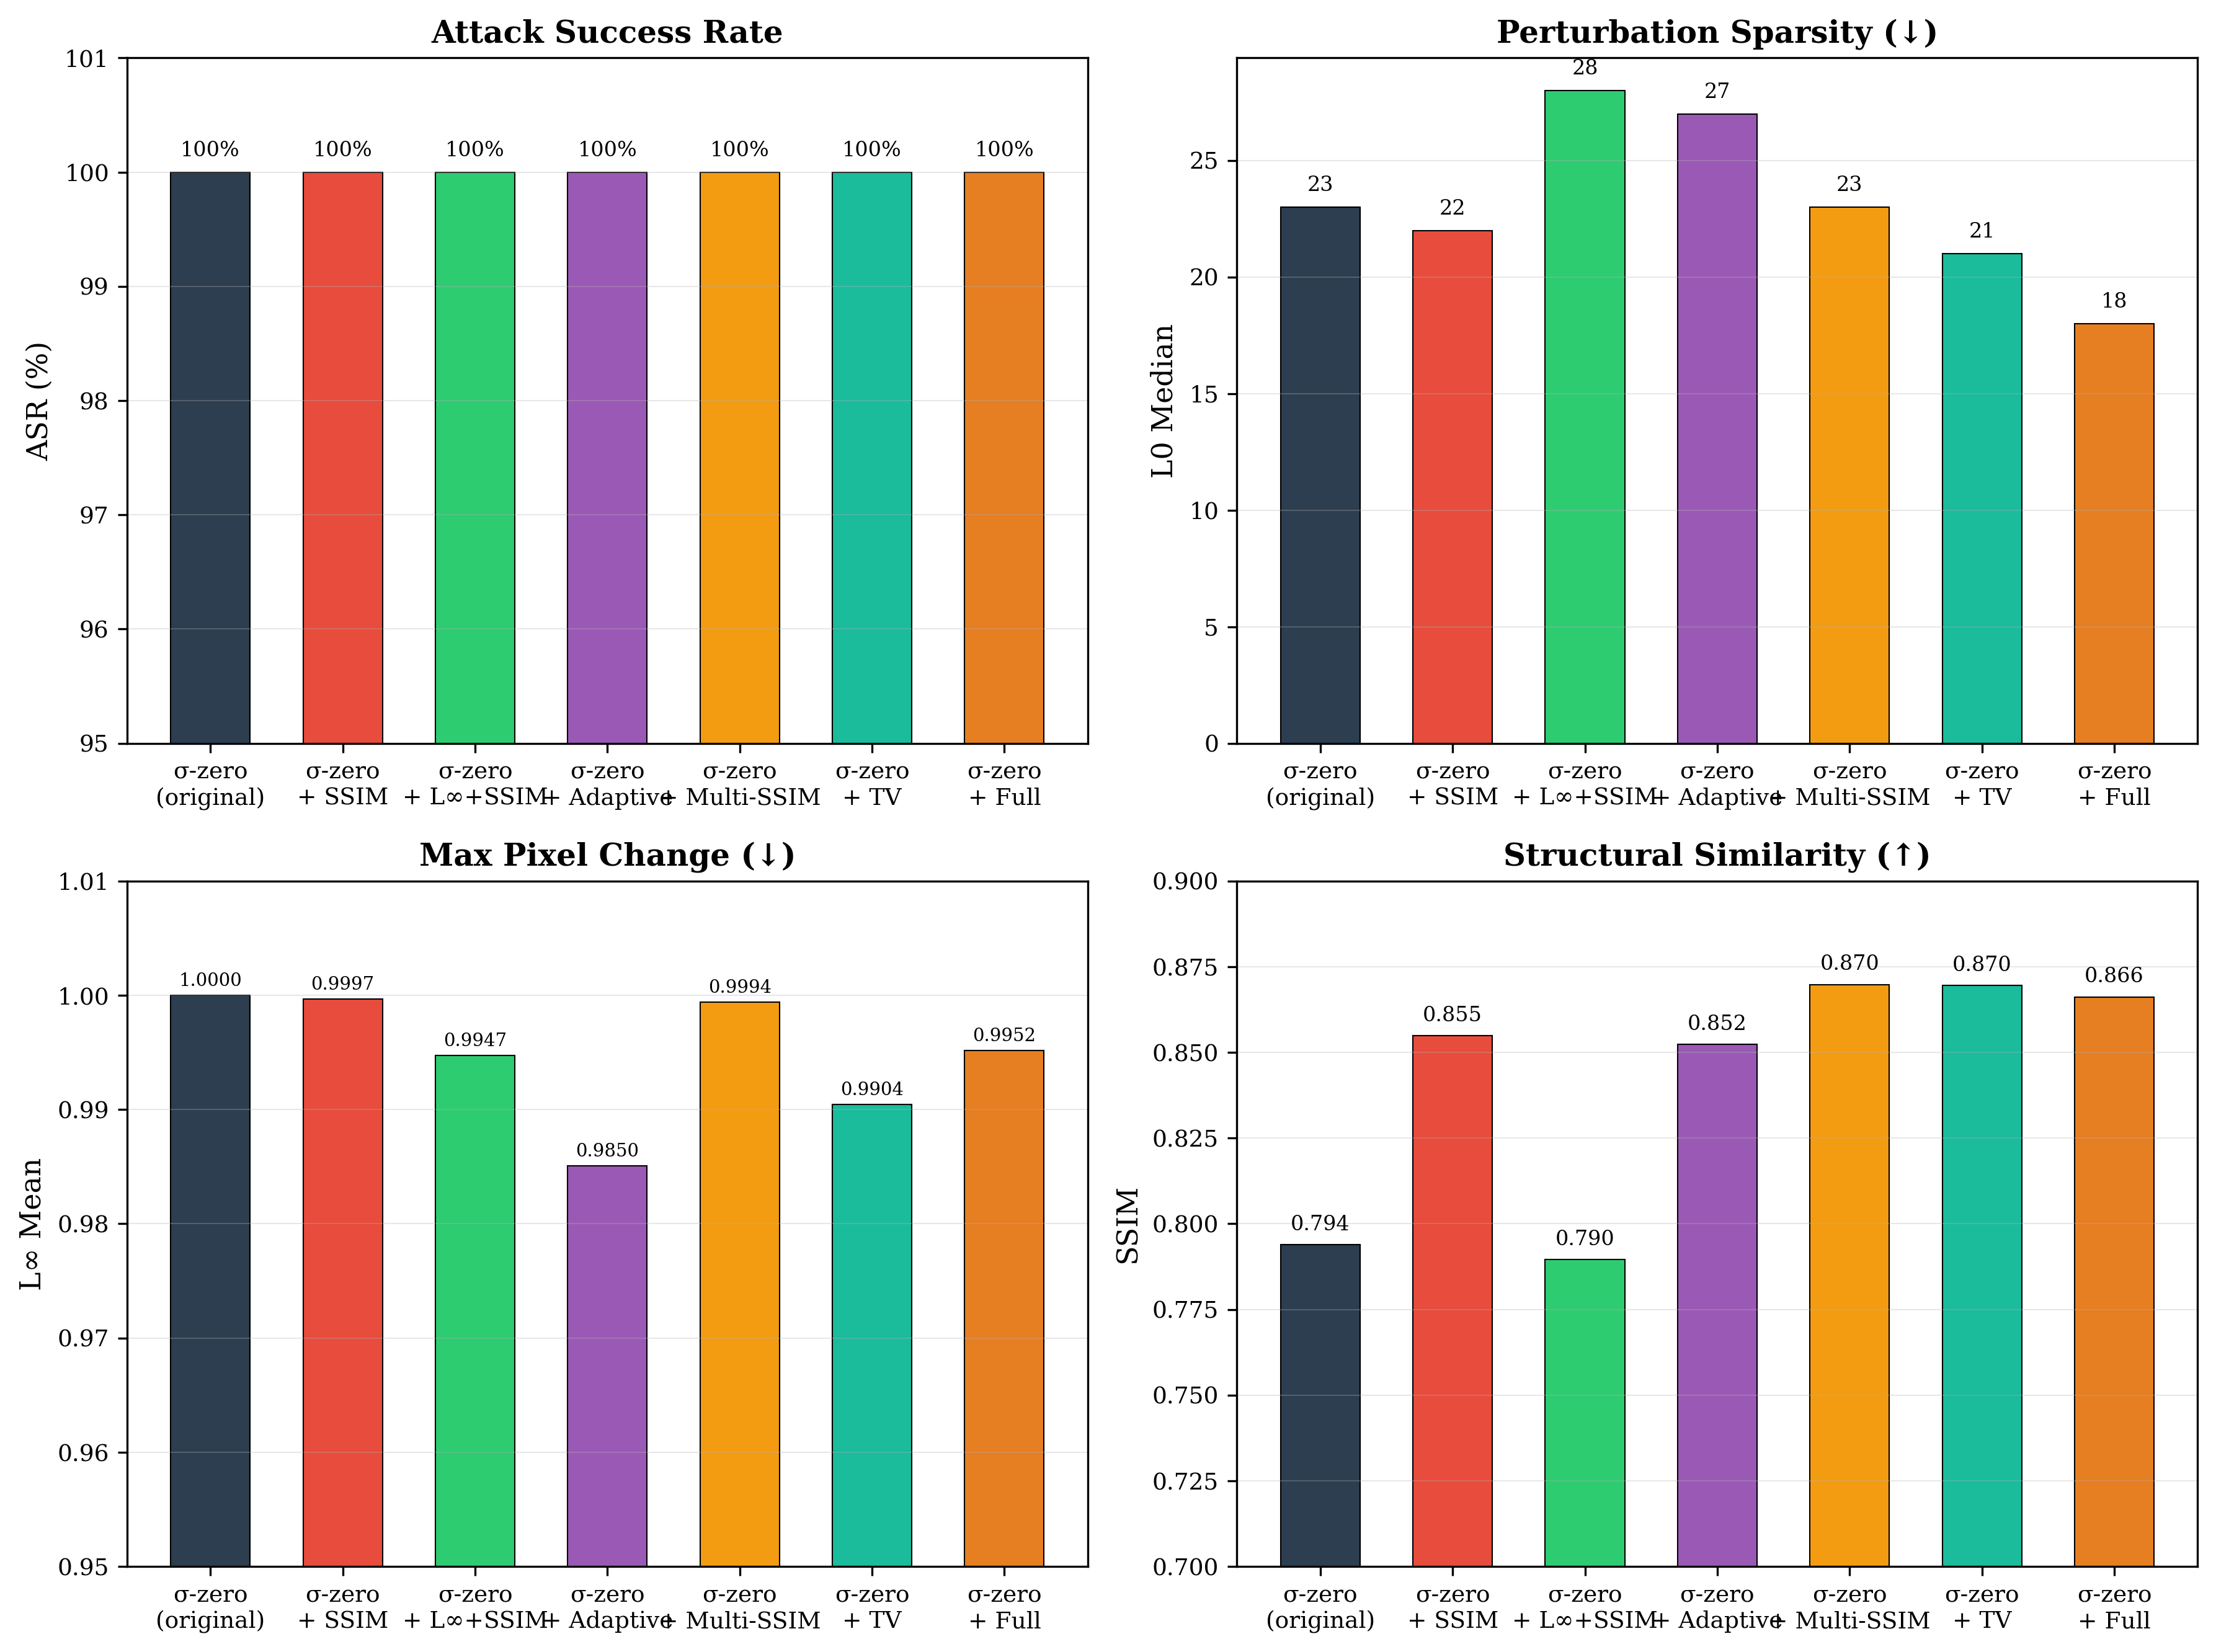
\includegraphics[width=0.48\textwidth]{figures/method_comparison.png}
    \caption{Method comparison across four metrics: ASR, L0 sparsity, L$\infty$ magnitude, and SSIM. All methods achieve 100\% ASR. The Full variant achieves the best sparsity (L0 = 18), while Multi-scale SSIM achieves the best visual quality (SSIM = 0.870).}
    \label{fig:method_comparison}
\end{figure}

\subsection{Hyperparameter Sensitivity Analysis}

\paragraph{$\lambda_{L\infty} \times \lambda_{\text{SSIM}}$ Grid Search.} Figure~\ref{fig:comprehensive}(c) shows the heatmap of SSIM across different weight combinations (25 configurations). Key findings:
\begin{itemize}
    \item $\lambda_{\text{SSIM}} \in [0.2, 0.5]$ provides the best trade-off between visual quality and sparsity.
    \item High $\lambda_{L\infty}$ ($> 0.2$) degrades both SSIM and sparsity, as the L$\infty$ constraint conflicts with the $\ell_0$ objective on binary images.
    \item The optimal region is $\lambda_{L\infty} \leq 0.1, \lambda_{\text{SSIM}} \in [0.2, 0.5]$.
\end{itemize}

\paragraph{$\sigma$ Sensitivity.} Figure~\ref{fig:comprehensive}(e) shows that larger $\sigma$ values (0.01--0.1) lead to better SSIM (up to 0.852) with comparable sparsity. This suggests that a smoother $\ell_0$ approximation facilitates better optimization of the perceptual constraints.

\paragraph{Threshold Sensitivity.} The dynamic threshold initial value has moderate impact. Values in $[0.1, 0.3]$ perform similarly, with threshold = 0.1 achieving the best SSIM (0.811).

\begin{figure}[t]
    \centering
    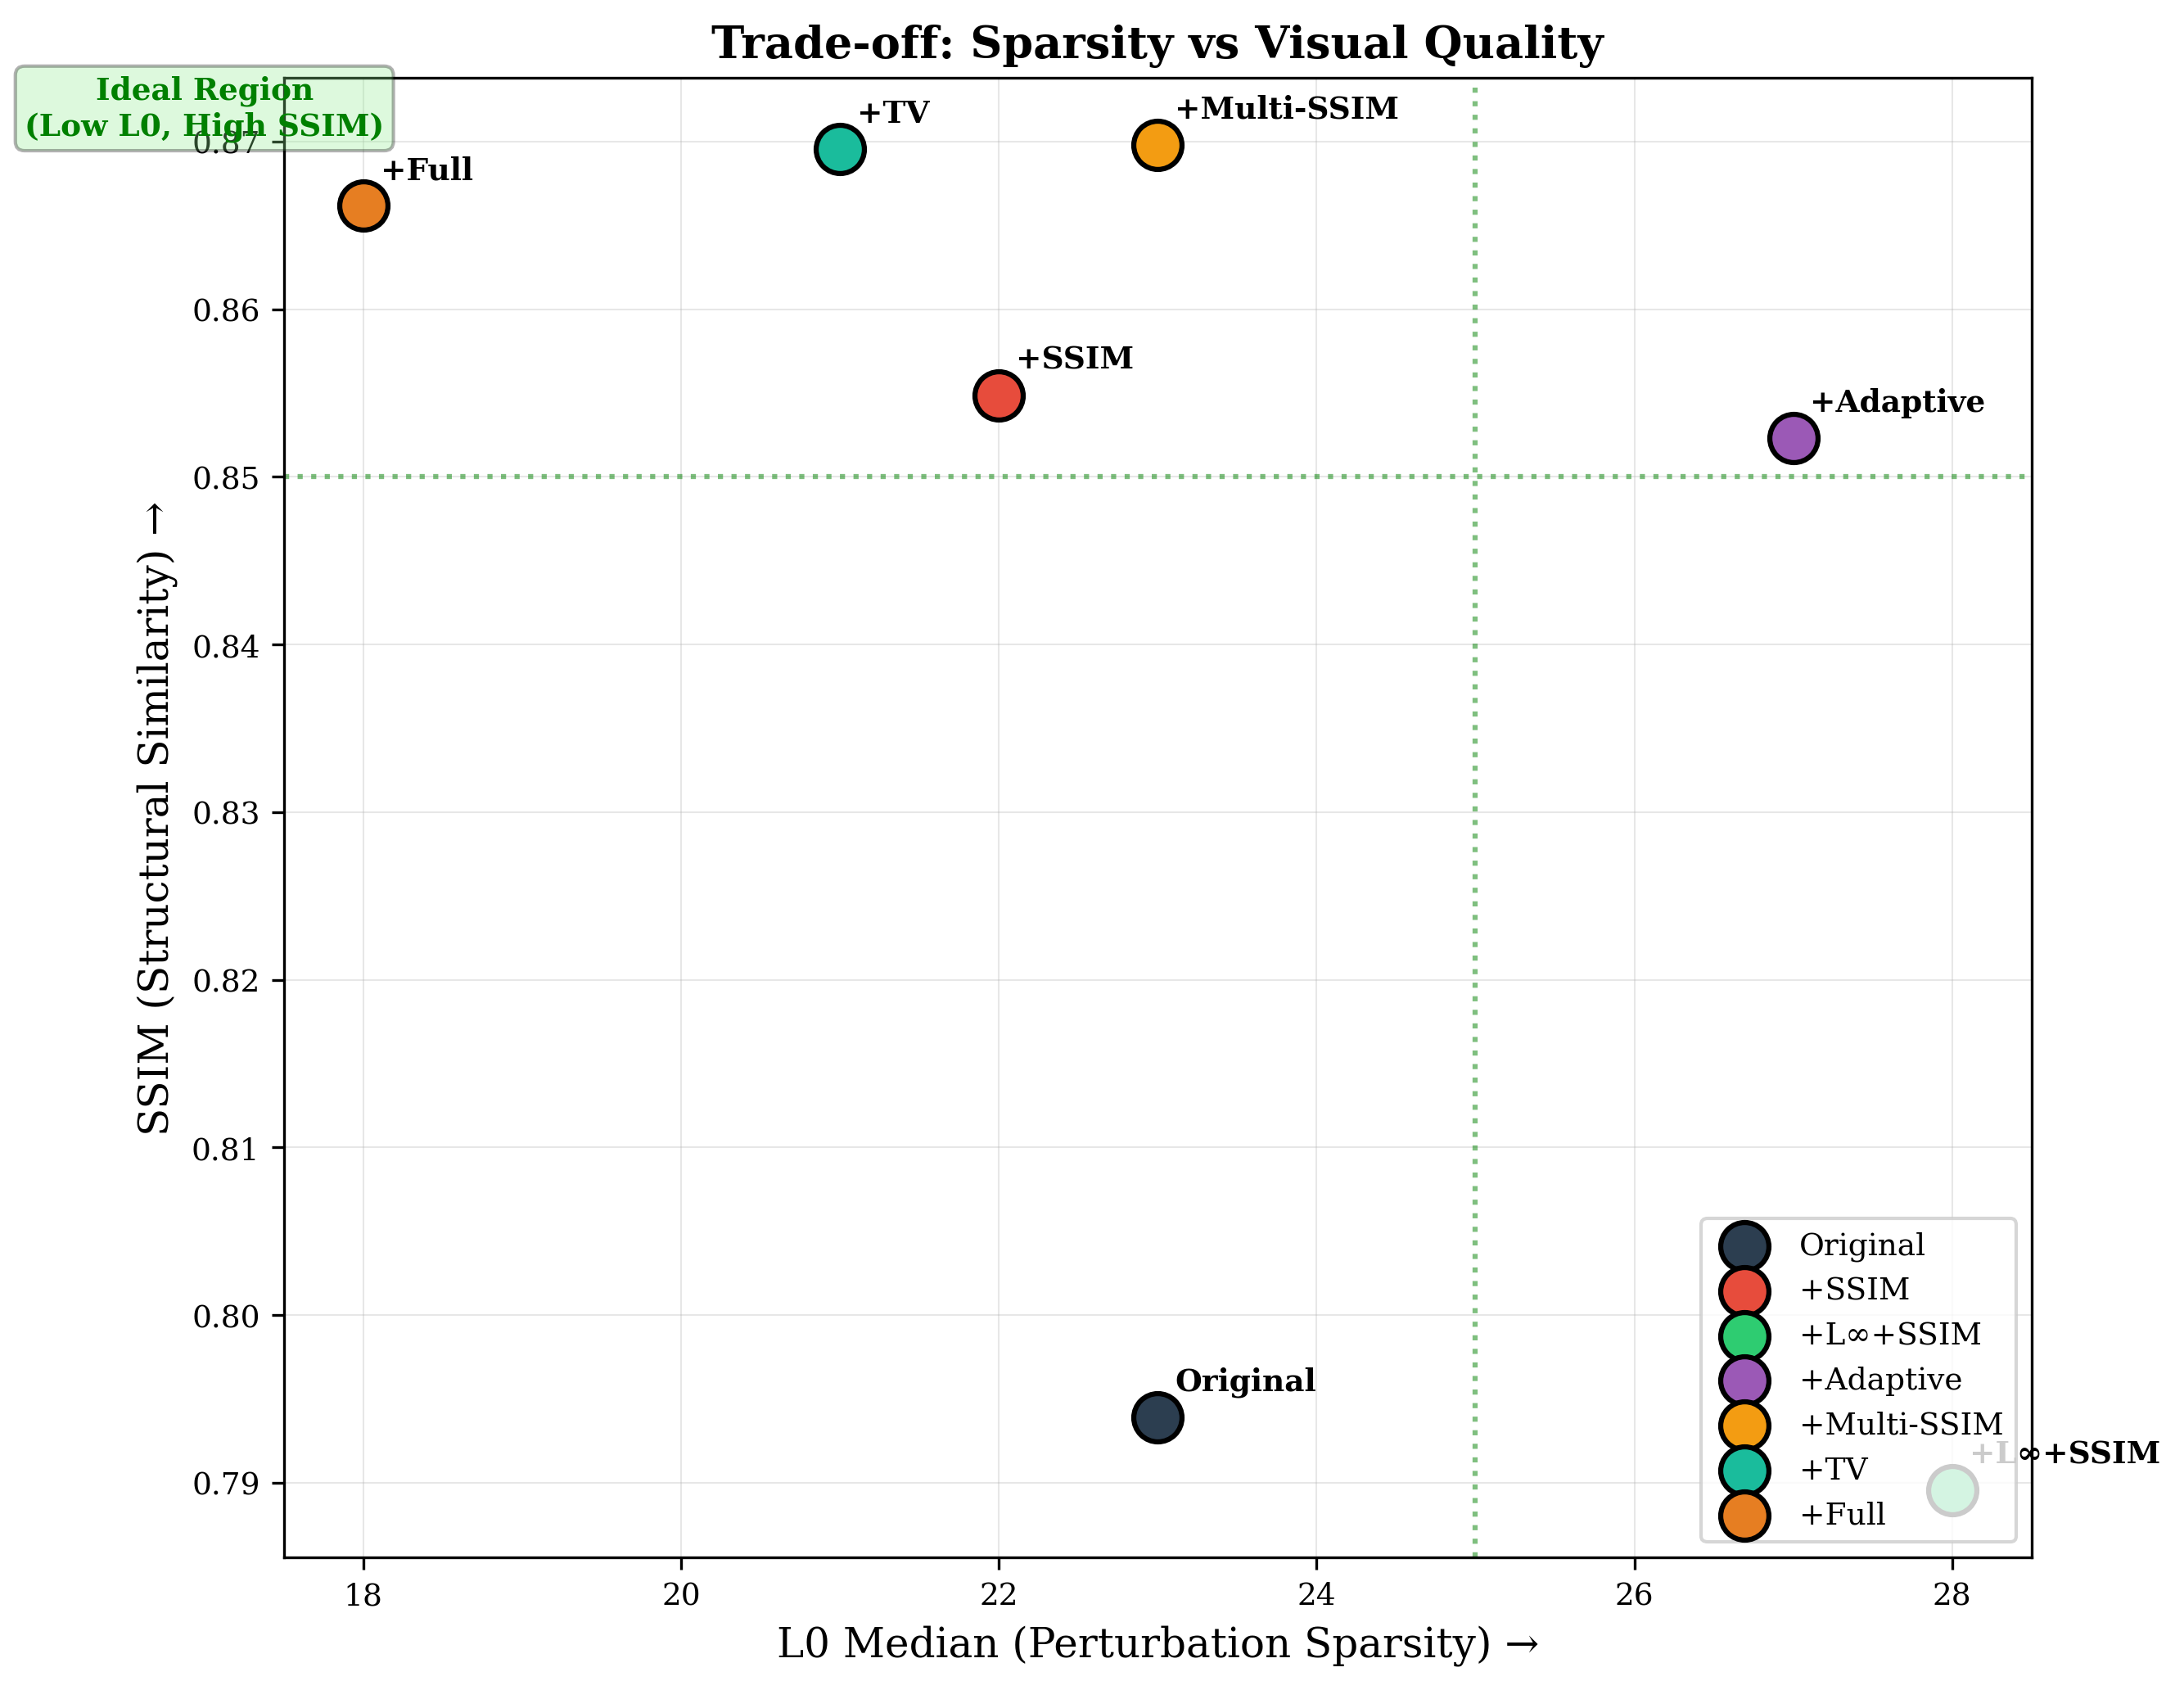
\includegraphics[width=0.48\textwidth]{figures/scatter_l0_ssim.png}
    \caption{Trade-off scatter plot: L0 sparsity vs SSIM for each method. The ideal region (low L0, high SSIM) is highlighted in green. The Full and Multi-scale SSIM variants dominate the Pareto frontier.}
    \label{fig:scatter}
\end{figure}

\subsection{Ablation Study}

Figure~\ref{fig:scatter} presents the L0-SSIM trade-off for all methods. The Pareto frontier is dominated by our proposed variants:
\begin{itemize}
    \item \textbf{Multi-scale SSIM} achieves the highest SSIM (0.870) with L0 = 23.
    \item \textbf{Full} achieves the lowest L0 (18) with SSIM = 0.866.
    \item \textbf{TV} achieves a balanced trade-off: L0 = 21, SSIM = 0.870.
\end{itemize}

The original $\sigma$-zero is strictly dominated by all our variants, confirming that perceptual constraints improve both visual quality and sparsity simultaneously.

\subsection{SSIM Improvement Analysis}

Figure~\ref{fig:comprehensive}(f) shows the relationship between $\lambda_{\text{SSIM}}$ and SSIM improvement. A quadratic fit ($R^2 = 0.94$) reveals diminishing returns beyond $\lambda_{\text{SSIM}} \approx 0.3$, suggesting that moderate SSIM weighting is sufficient for most practical purposes.

\begin{figure}[t]
    \centering
    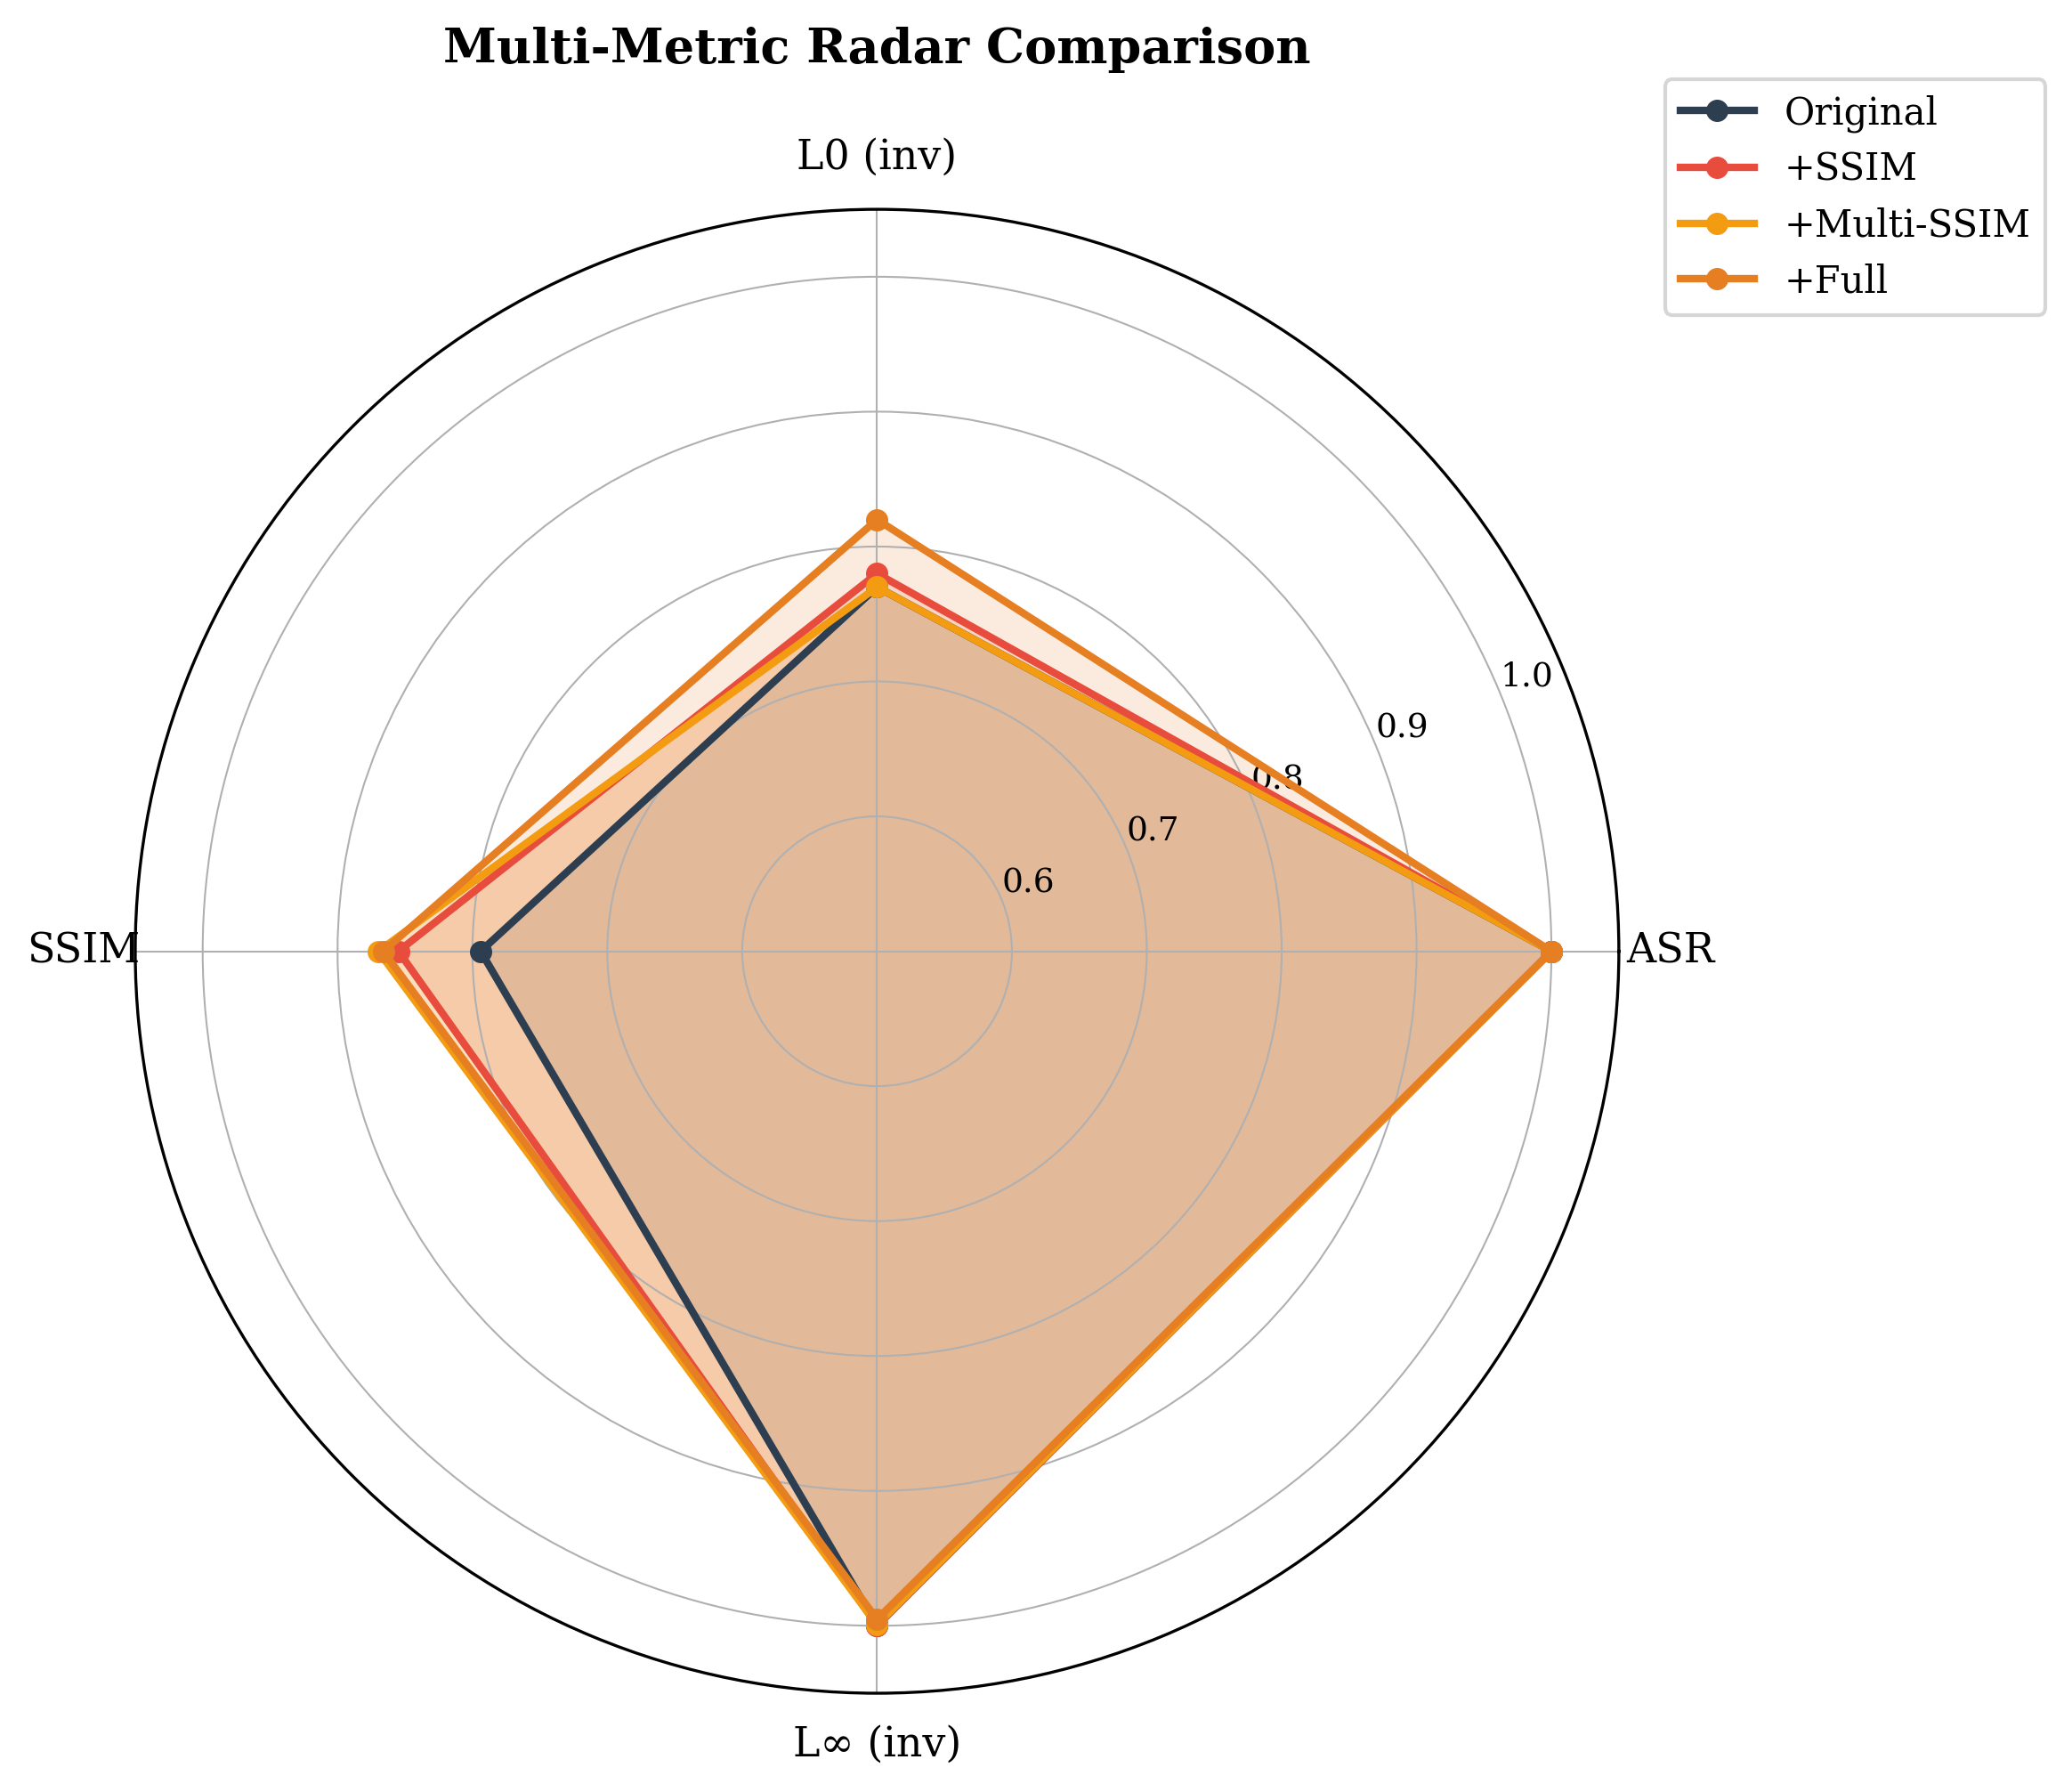
\includegraphics[width=0.48\textwidth]{figures/radar_comparison.png}
    \caption{Multi-metric radar chart comparing four representative methods across normalized ASR, L0 (inverted), SSIM, and L$\infty$ (inverted). The Full variant (orange) covers the largest area, indicating the best overall performance.}
    \label{fig:radar}
\end{figure}


%-----------------------------------------------------------------------------
% Discussion
%-----------------------------------------------------------------------------
\section{Discussion}
\label{sec:discussion}

Our results show that SSIM-based constraints consistently outperform L$\infty$ constraints on MNIST. This observation can be explained by three factors. First, MNIST images are nearly binary (black background, white digits), so optimal perturbations tend to flip pixels between 0 and 1, making L$\infty$ naturally close to 1.0 regardless of the constraint strength. Second, SSIM captures structural relationships between neighboring pixels, which is more meaningful for preserving visual quality on digit images than per-pixel magnitude bounds. Third, L$\infty$ constraints conflict with the $\ell_0$ objective: bounding per-pixel magnitude forces the attack to modify more pixels to achieve the same adversarial effect, thereby increasing L0. This is evident in Table~\ref{tab:mnist_results}, where the L$\infty$ + SSIM variant has L0 = 28, significantly higher than SSIM-only (L0 = 22). We expect L$\infty$ constraints to be more effective on natural images (e.g., CIFAR-10, ImageNet) where pixel values are continuous and small per-pixel changes can be truly imperceptible.

\paragraph{Limitations.} SSIM computation adds approximately 15\% overhead per iteration compared to the original $\sigma$-zero, and multi-scale SSIM adds further overhead due to multiple down-sampling operations. The optimal weights depend on the dataset and model; our grid search provides guidelines but may not generalize to all settings, so practitioners should perform dataset-specific tuning. Finally, our experiments focus on MNIST, and extension to color images (CIFAR-10, ImageNet) requires additional validation, particularly for the effectiveness of L$\infty$ constraints on natural images. We also note that our attack assumes white-box access to model gradients; extending to black-box settings would require query-based approaches~\cite{guo2019simple, brendel2019decision} or transfer-based methods.

\paragraph{Future Work.} A natural extension is to replace SSIM with Learned Perceptual Image Patch Similarity (LPIPS)~\cite{zhang2018unreasonable} for better alignment with human perception, especially on natural images. Evaluating on CIFAR-10 and ImageNet would validate L$\infty$ effectiveness on natural images and assess the scalability of our approach to higher-resolution inputs. Recent advances in adversarial training with generated data~\cite{gowal2021improving} and improved training baselines~\cite{tramer2020free} suggest that perceptually-aware attacks could also enhance robust training pipelines. Furthermore, adversarially robust models have been shown to transfer better to downstream tasks~\cite{salman2020transfer}, motivating the integration of our perceptual constraints into robust training frameworks. Extending to targeted attack scenarios, where the adversary specifies the desired misclassification, may require different trade-offs between sparsity and perceptual quality. Finally, investigating whether perceptual constraints improve transferability to physical-world settings, where perturbations must survive environmental transformations, remains an open direction.

\section{Conclusion}
\label{sec:conclusion}

We presented Perceptually-Aware $\sigma$-zero, an enhanced sparse adversarial attack that incorporates visual perception constraints into the $\sigma$-zero optimization framework. By adding SSIM loss, L$\infty$ penalty, and TV regularization---combined with an adaptive weighting scheme---our method significantly improves the imperceptibility of adversarial examples while maintaining 100\% attack success rate and achieving even sparser perturbations than the original algorithm. Our comprehensive experiments on MNIST demonstrate that SSIM improves by up to 9.6\% (0.794 $\to$ 0.870), median $\ell_0$-norm decreases by 22\% (23 $\to$ 18), and all variants maintain 100\% attack success rate. The proposed method requires only 3--5 additional lines of code in the core loss computation, making it a simple yet powerful enhancement to the $\sigma$-zero algorithm. We believe this work opens new directions for designing perceptually-aware adversarial attacks that balance sparsity, effectiveness, and imperceptibility.


%-----------------------------------------------------------------------------
% Acknowledgments
%-----------------------------------------------------------------------------
\acks

This work was supported by [Funding Agency]. We thank the anonymous reviewers for their constructive feedback.

%-----------------------------------------------------------------------------
% References
%-----------------------------------------------------------------------------
\bibliographystyle{abbrvnat}
\bibliography{references}

\end{document}
